\section{Characterization}
    %%%%%%%%%%%%%%%%%%%%%%%%%%%%%%%%%%%%%
	%%  Slide 1: <> %%
	%%%%%%%%%%%%%%%%%%%%%%%%%%%%%%%%%%%%%
    \begin{frame}
        \frametitle{Threshold and noise}\medskip
        The lower the threshold, the lower the minium detectable signal, allowing for thinner detector (Q$_{MIP}\propto$d). \\
        \medskip
        The threshold and the noise are \textbf{strictly} related with the \textbf{FE} settings\\
        \medskip
        What determins the minimum stable threshold?
        \begin{itemize}
            \item the \textbf{ENC} = Equivalent Noise Charge
            \item the \textbf{threshold dispersion} among different pixels
        \end{itemize}
        \medskip
        \centering ......................................................................\\\medskip
        \centering Expected values found by simulation with optimal FE settings %(sottolinea NON DA ME)
        \begin{center}
        \begin{beamercolorbox}[rounded=true, center]{palette light primary}
            Noise \hspace*{1.2cm} Threshold \hspace*{1.2cm} Threshold dispersion
        \end{beamercolorbox}
        \begin{beamercolorbox}[rounded=true, center]{palette titleframe}
            \hspace*{-2.4cm} $\sim$\SI{9}{\elementarycharge}$^-$ \hspace*{1.4cm} $\sim$\SI{270}{\elementarycharge}$^-$ \hspace*{1.2cm} $\sim$\SI{30}{\elementarycharge}$^-$
        \end{beamercolorbox}
    \end{center}
    \end{frame}


    %%%%%%%%%%%%%%%%%%%%%%%%%%%%%%%%%%%%%
	%%  Slide 1: <Scurve> %%
	%%%%%%%%%%%%%%%%%%%%%%%%%%%%%%%%%%%%%
    \begin{frame}
        \frametitle{Threshold and noise: how to measure them?}
        \begin{itemize}
            \item\textbf{Internal injection circuit} allows sending a voltage step V$_{inj}$[DAC] on an injection capacitance C$_{inj}$ at the FE input\\\medskip
            \item Scan at different pulse height V$_{inj}$[DAC] injecting 100 pulses at fixed discriminator threshold 
        \end{itemize}
        \medskip\medskip
        By design:
        \begin{beamercolorbox}[ rounded=true, center]{palette light primary}
            C$_{inj}$ = \SI{230}{fF} $\rightarrow$ Q$_{inj}$ = \SI{20}{\elementarycharge}$^-$/DAC
        \end{beamercolorbox}  
    \end{frame}


    %%%%%%%%%%%%%%%%%%%%%%%%%%%%%%%%%%%%%
	%%  Slide 1: <Scurve> %%
	%%%%%%%%%%%%%%%%%%%%%%%%%%%%%%%%%%%%%
    \begin{frame}
        \frametitle{S-curve}
        \begin{itemize}
            \item Efficiency curve as a function of the injected V$_{inj}$[DAC]
        \end{itemize}
        \medskip
        \begin{columns}
            \column{0.45\textwidth}  
                \includegraphics[width=1.1\linewidth]{figures/charaterization/s_curve_presentazione.pdf}
            \column{0.55\textwidth} 
                Assuming a gaussian noise:
                \begin{itemize}
                    \item threshold $\rightarrow$ the 50\%
                    \item noise $\rightarrow$ 1/slope 
                \end{itemize}
                \medskip
                Analytical parametrization of the curve with the $error\,function$\\
                
   
                %\begin{equation*}
                %    \tiny
                %    f(x, \mu, \sigma) = \frac{1}{2} \; \left(1\,+\,erf\left(\frac{x-\mu}{\sigma \sqrt{2}}\right)\right)
                %    \label{eq:fit_scurve}
                %\end{equation*}
        \end{columns} 
        \begin{beamercolorbox}[ rounded=true, center]{palette titleframe}
            Q$_{inj}$=\SI{20}{\elementarycharge}$^-$/DAC
        \end{beamercolorbox}
    \end{frame}



    %%%%%%%%%%%%%%%%%%%%%%%%%%%%%%%%%%%%%%%%
    %%  Slide 2: <Threshold_noise>  %%
    %%%%%%%%%%%%%%%%%%%%%%%%%%%%%%%%%%%%%%%%
    \begin{frame}
        \frametitle{Threshold and noise results}
        \bigskip
        \begin{columns}
            \column{0.45\textwidth}        
                \includegraphics[width=.95\linewidth]{figures/charaterization/threshold_PMOSB.pdf}
            \column{0.45\textwidth}        
                \includegraphics[width=.95\linewidth]{figures/charaterization/noise_PMOSB.pdf} 
        \end{columns}                  
        %\hspace*{+0.1cm}
        \begin{columns}
            \column{0.45\textwidth} 
                \begin{table}[h!]
                    \footnotesize
                    \begin{tabular}{| c |  c | c|}
                    \hline
                    & Measurement & Simulation \\
                    \hline
                    \hline
                    $\mu$ [\si{\elementarycharge}$^-$] & 400.8$\pm$0.2 & $\sim$270\\
                    $\Delta_{\mu}$ [\si{\elementarycharge}$^-$] & 33.0$\pm$0.2 & $\sim$30\\
                    $\sigma$ [\si{\elementarycharge}$^-$] & 12.26$\pm$0.07 & $\sim$9 \\
                    $\Delta_{\sigma}$ [\si{\elementarycharge}$^-$] & 1.50$\pm$0.05 & -\\
                    \hline
                    \end{tabular}
                \end{table}       
            \column{0.1\textwidth} 

            \column{0.45\textwidth} 
                Noise rate with this FE setting $\sim$\SI{3}{Hz} 
        \end{columns}

        \end{frame}



    %%%%%%%%%%%%%%%%%%%%%%%%%%%%%%%%%%%%%%%%
    %%  Slide 4: <ToT vs charge>  %%
    %%%%%%%%%%%%%%%%%%%%%%%%%%%%%%%%%%%%%%%%
    \begin{frame}
        \frametitle{Calibration of the signal}
        How convert the $ToT_{signal, clk}$ in electrons?
        \smallskip
        \pause
        \begin{enumerate}
            \item Used the \textbf{internal injection} circuit for a parametrization of the ToT: $ToT_{signal,clk}\rightarrow V_{signal, DAC}$
            \item Used radioactive source for a reference in charge $e^-$: $V_{signal, DAC}\rightarrow Q_{signal, e^-}$
        \end{enumerate}
        \medskip
        \pause
        \begin{beamercolorbox}[sep=0em,wd=0.95\textwidth,ht=1.5ex, dp=0.1ex, rounded=true, center]{palette light primary}
            Fe$^{55}$ $\rightarrow$ Mn$^{55}$ + K$_\alpha$ (\SI{5.9}{keV}, 24.4\%) or K$_\beta$ (\SI{6.5}{keV}, 2.9\%)
        \end{beamercolorbox}
        \begin{tikzpicture}[overlay]
            \draw[decorate,decoration={brace}]
                (3.5,0) -- (5.5,0);
        \end{tikzpicture}
        \begin{columns}
            \column{0.2\textwidth}    
            \column{0.8\textwidth}    
            \begin{itemize}
                \item P$_{abs, photo-electric}\sim$58\% $\rightarrow$ $\lambda$=\SI{29}{\um}
                \item $w_i$=\SI{3.6}{eV} in Si @ \SI{300}{\kelvin}$\rightarrow$ \SI{1616}{\elementarycharge}$^-$
            \end{itemize}
        \end{columns}
        \medskip
        \pause
        \begin{beamercolorbox}[rounded=true, center]{palette titleframe}
        \begin{equation*}
            Q_{signal,e^-} = \frac{1616e^-}{V_{Fe55,DAC}}V_{signal,DAC}=\frac{1616e^-}{V_{Fe55,DAC}}\frac{(ToT_{signal,clk}-q)}{slope}
        \end{equation*}
    \end{beamercolorbox}
    \end{frame}  



    %%%%%%%%%%%%%%%%%%%%%%%%%%%%%%%%%%%%%%%%
    %%  Slide 3: <ToT linearity>  %%
    %%%%%%%%%%%%%%%%%%%%%%%%%%%%%%%%%%%%%%%%
    \begin{frame}
        \frametitle{ToT calibration}
        \begin{itemize}
            \item ToT[clock counts] calibration in V$_{inj, DAC}$ done using the internal \textbf{injection} circuit
            \item Scan in the voltage step height V$_{inj, DAC}$
            \item Q$_{inj,e^-}$ depends on the C$_{inj}$, different for each pixel: Q$_{inj}$=V$_{inj}$C$_{inj}$\\  
            %\item Sent 100 pulse for each V$_{inj, ToT}$[DAC]
        \end{itemize}
        %\begin{beamercolorbox}[rounded=true, center]{palette titleframe}
        %    \begin{equation*}
        %        ToT[clk.cnts] = V_{inj, ToT}[DAC] slope[DAC/clk.cnts] + q[clk.cnts]
        %    \end{equation*}
        %\end{beamercolorbox}
        \medskip
        \begin{columns}
            \column{0.5\textwidth}  
                \includegraphics[width=0.95\linewidth]{figures/Monopix1/pulse_60to10.png}
            \column{0.5\textwidth}
                \includegraphics[width=1.\linewidth]{figures/charaterization/tot_presentazione.pdf} 
        \end{columns}
    \end{frame}    

    %%%%%%%%%%%%%%%%%%%%%%%%%%%%%%%%%%%%%%%%
    %%  Slide 4: <ToT calibration>  %%
    %%%%%%%%%%%%%%%%%%%%%%%%%%%%%%%%%%%%%%%%
    \begin{frame}
        \frametitle{ToT absolute calibration: Fe$^{55} \rightarrow$ Mn$^{55}$ K$_{\alpha}$}
        \begin{columns}
            \column{0.65\textwidth} 
            \centering
           % Single pixel distribution of the ToT
            \begin{itemize}
                \item Single pixel distribution of the ToT
            \end{itemize}
                \hspace*{+0.3cm}\includegraphics[width=1.45\linewidth]{figures/charaterization/absolute_calibration_explanation.pdf}
            \column{0.5\textwidth} 
            \vspace*{2.5cm} 
            %For each pixel in the matrix:
            \begin{enumerate}
                \item Fit with a \textbf{gaussian} to find the peak position in the spectrum
                \item Conversion from ToT to DAC (using the line parameters)
                \item Peak value in DAC fixed to be equal to \SI{1616}{\elementarycharge}$^-$
            \end{enumerate} 
        \end{columns}
    \end{frame}     



    %%%%%%%%%%%%%%%%%%%%%%%%%%%%%%%%%%%%%%%%
    %%  Slide 4: <ToT calibration>  %%
    %%%%%%%%%%%%%%%%%%%%%%%%%%%%%%%%%%%%%%%%
    \begin{frame}
        \frametitle{Calibration results}
        \begin{columns}
            \column{0.5\textwidth} 
            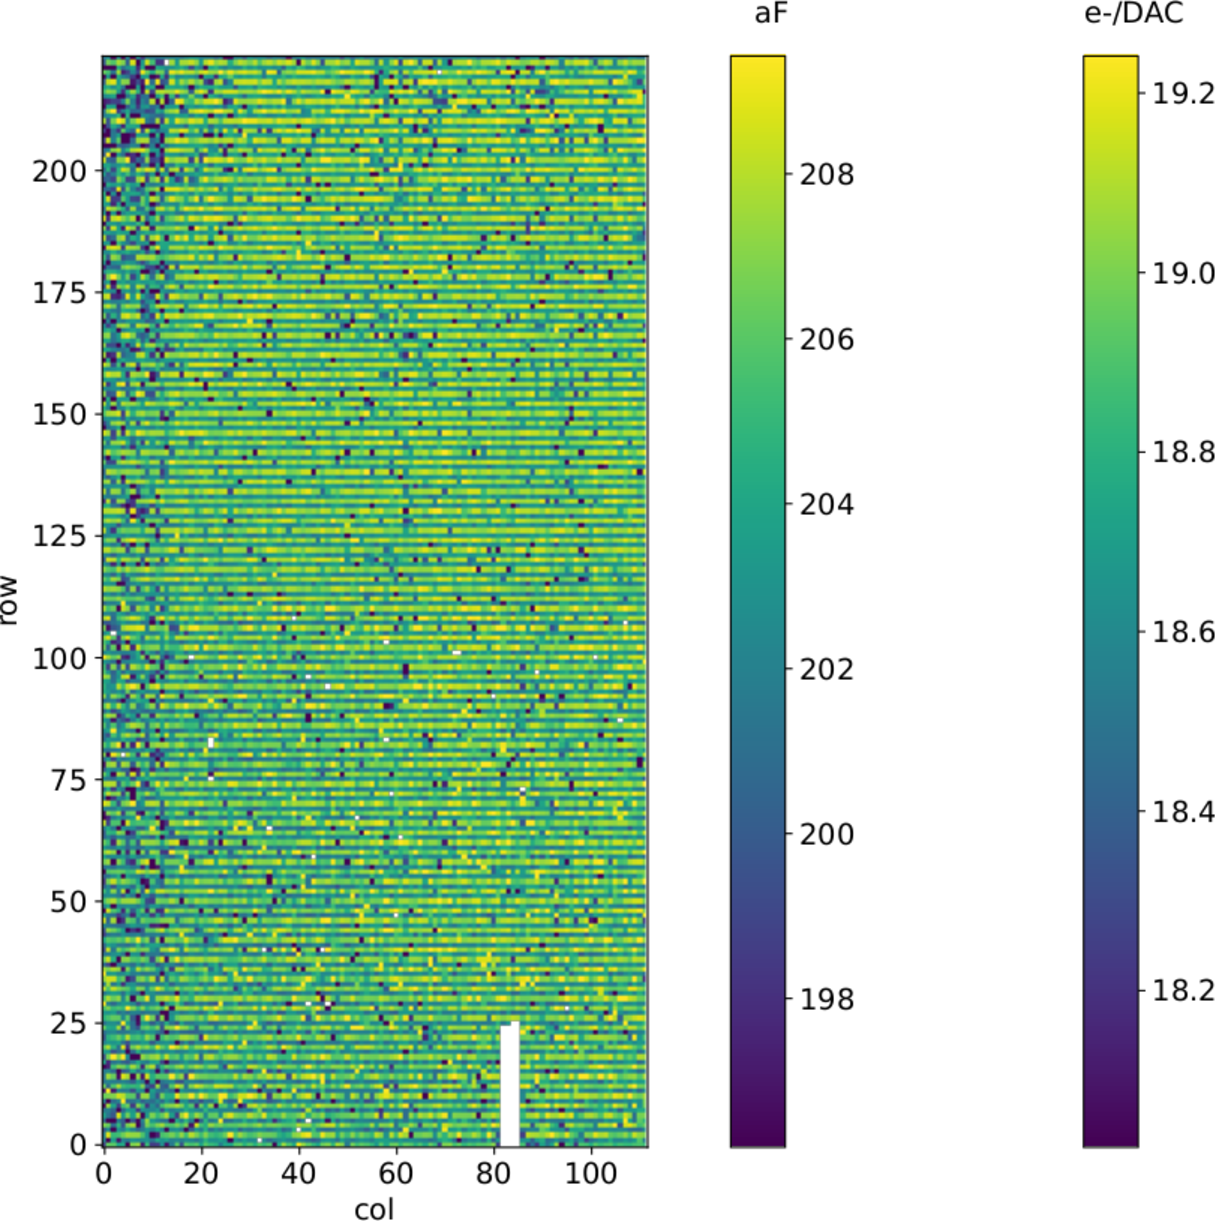
\includegraphics[width=1.1\linewidth]{figures/charaterization/conversion_factor_map.pdf}
            \column{0.5\textwidth} 
            \begin{itemize}
                \item C$_{inj}$ is in range 180-200\si{fF} (expected \SI{230}{fF})
                \item F is is range 16.5-18.5 (expected \SI{20.2}{\elementarycharge/DAC}$^-$)
                \item structure on rows probably due to bias line differences in the injection circuit 
                \item applying the calibration the threshold and noise are respectively \SI{340}{\elementarycharge}$^-$ and \SI{10}{\elementarycharge}$^-$
            \end{itemize}
        \end{columns}
    \end{frame}


    %%%%%%%%%%%%%%%%%%%%%%%%%%%%%%%%%%%%%%%%
    %%  Slide 5: <ToT bias>  %%
    %%%%%%%%%%%%%%%%%%%%%%%%%%%%%%%%%%%%%%%%
    \begin{frame}
        \frametitle{Changing the bias}
        \begin{columns}
            \column{0.28\textwidth} 
                Acquisitions with:
                \begin{itemize}
                    \item Injection
                    \item Fe$^{55}$ source
                \end{itemize}
            \column{0.8\textwidth} 
                %Maximum bias suggested
                \begin{table}
                    \begin{center}
                    \scalebox{0.85}{
                    \begin{tabular}{| c |  c | c | c |}
                    \hline
                    & -\SI{6}{V} & -\SI{3}{V} & \SI{0}{V}\\
                    \hline
                    \hline
                    Threshold [DAC] & 20 $\pm$ 2 & 21 $\pm$ 2 & 24 $\pm$ 2\\
                    Noise [DAC] & 0.61 $\pm$ 0.08 & 0.62 $\pm$ 0.08 & 0.82 $\pm$ 0.1\\
                    \hline
                    \end{tabular}}
                    \end{center}
                \end{table}
        \end{columns}
        \begin{columns}
            \column{0.4\textwidth}  
            \medskip        
            \includegraphics[width=1.1\linewidth]{figures/charaterization/ToT_gain.pdf}
            \column{0.05\textwidth}

            \column{0.6\textwidth}
            Reducing the bias from -\SI{6}{V} to \SI{0}{V} reduction of the below quantity in the Fe$^{55}$ spectrum: 
            \begin{enumerate}
                \item ToT value of the peak $\sim$30\%
                \item N of events under the peak $\sim$60\%
                \item hit rate $\sim$60\%
            \end{enumerate}
            1 is due to the reduction in the gain, 2 and 3 are due to the decrease in the depletion thickness
        \end{columns}
    \end{frame}      




    %%%%%%%%%%%%%%%%%%%%%%%%%%%%%%%%%%%%%%%%
    %%  Slide 4: <Aquisitions with sources>  %%
    %%%%%%%%%%%%%%%%%%%%%%%%%%%%%%%%%%%%%%%%
    \begin{frame}
        \frametitle{Acquisition with Sr$^{90}$$\rightarrow$Y$^{90}$$\beta^-$$\rightarrow$Zr$^{90}$$\beta^-$}
        \begin{columns}
            \column{0.5\textwidth} 
                \begin{itemize}
                    \item Q released per pixel for different cluster sizes
                \end{itemize}
                \bigskip
                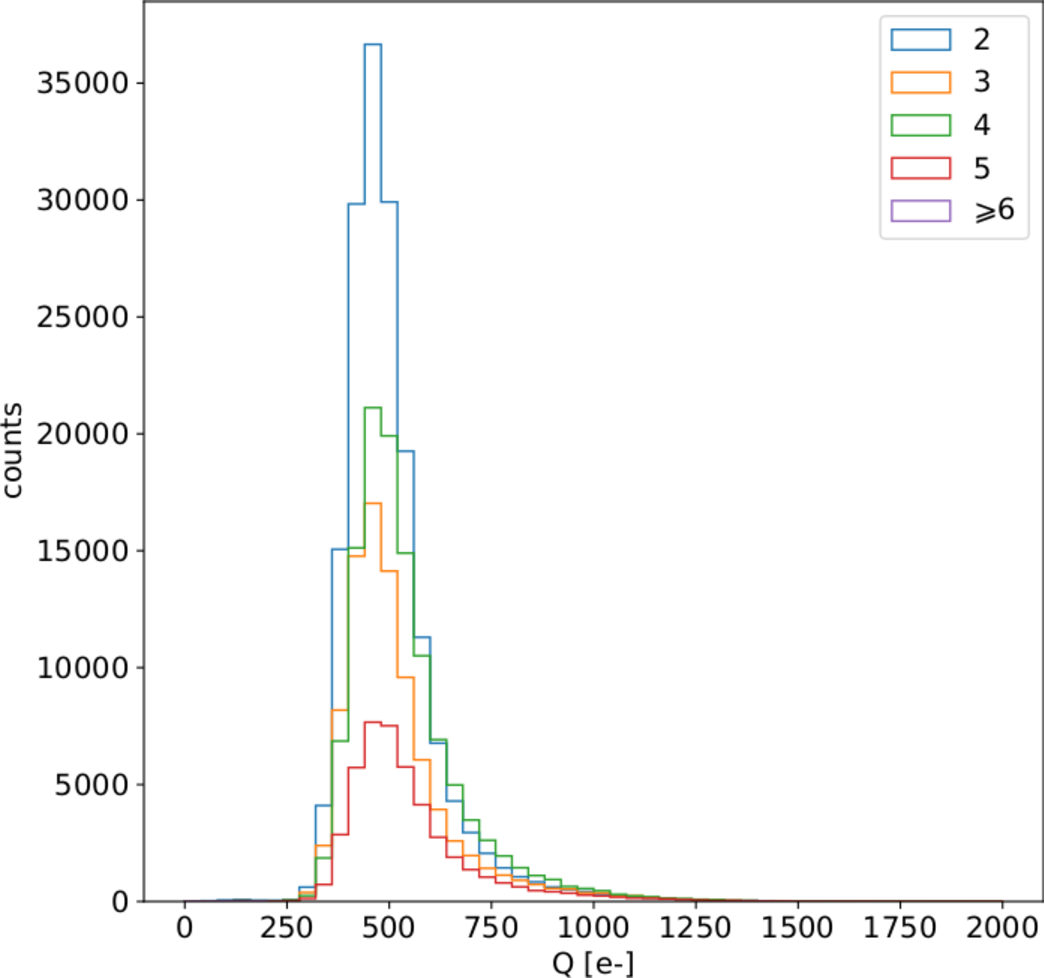
\includegraphics[width=1.1\linewidth]{figures/charaterization/Sr90_spectrum_per_pixel.pdf} 
            \column{0.5\textwidth} 
            %\vspace*{+1.4cm}
            %\begin{tikzpicture}[overlay]
            %    \draw[decorate,decoration={brace,mirror}](0.5,0) -- (1.5,0);
            %    \draw[decorate,decoration={brace,mirror}](3.,0) -- (3.,0);
            %\end{tikzpicture}
            %E$_{e, max}$=\SI{546}{keV}, 
            \centering\includegraphics[width=.75\linewidth]{figures/charaterization/large_angle_particles.pdf}
                \begin{figure}
                    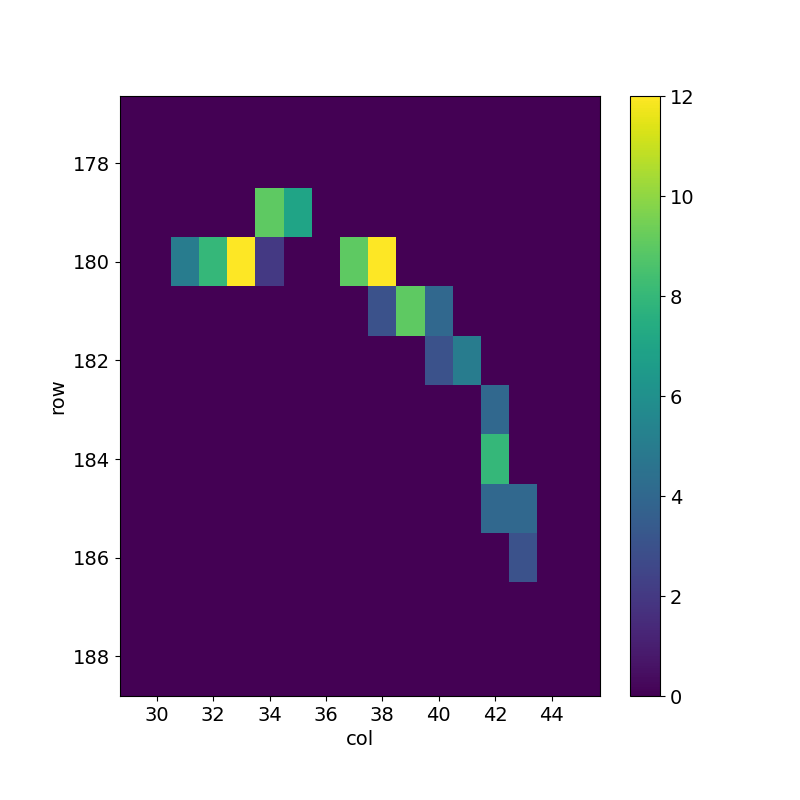
\includegraphics[width=.3\linewidth]{figures/charaterization/evts/Sr90/18b.png}
                    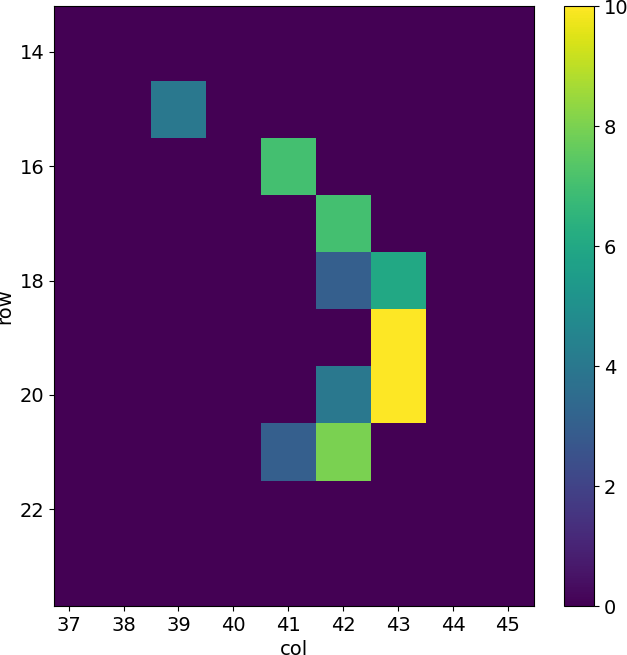
\includegraphics[width=.3\linewidth]{figures/charaterization/evts/Sr90/10b.png} 
                    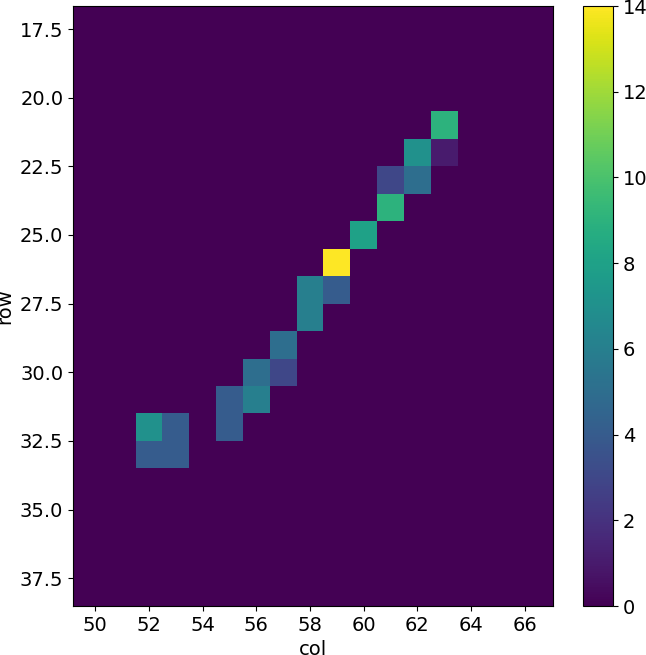
\includegraphics[width=.3\linewidth]{figures/charaterization/evts/Sr90/21a.png}
                \end{figure}
                \begin{itemize}
                    \item E$_{e, max}$=\SI{2.3}{MeV}
                    \item Q in cluster is proportional to the cluster size
                    \item due to large angle electrons
                    \item charge sharing among pixels 
                \end{itemize}
        \end{columns}
    \end{frame}    

    %%%%%%%%%%%%%%%%%%%%%%%%%%%%%%%%%%%%%%%%
    %%  Slide 4: <Aquisitions with sources>  %%
    %%%%%%%%%%%%%%%%%%%%%%%%%%%%%%%%%%%%%%%%
    \begin{frame}
        \frametitle{Acquisition with cosmic rays}
        \begin{columns}
            \column{0.5\textwidth} 
                \begin{itemize}
                    \item Q released per pixel for different cluster sizes 
                \end{itemize}
                \bigskip
                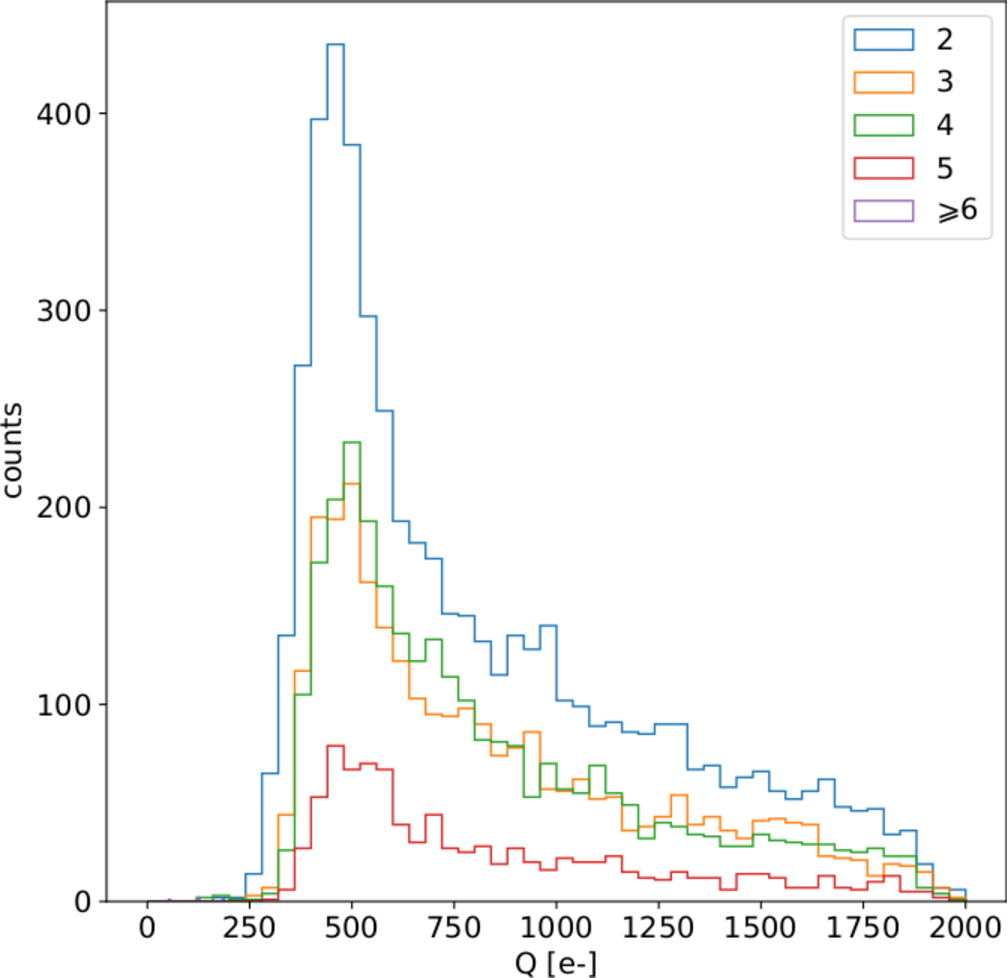
\includegraphics[width=1.1\linewidth]{figures/charaterization/cosmic_rays_spectrum_per_pixel.pdf} 
            \column{0.5\textwidth} 
            \centering\includegraphics[width=.75\linewidth]{figures/charaterization/large_angle_particles.pdf}
                \begin{figure}
                    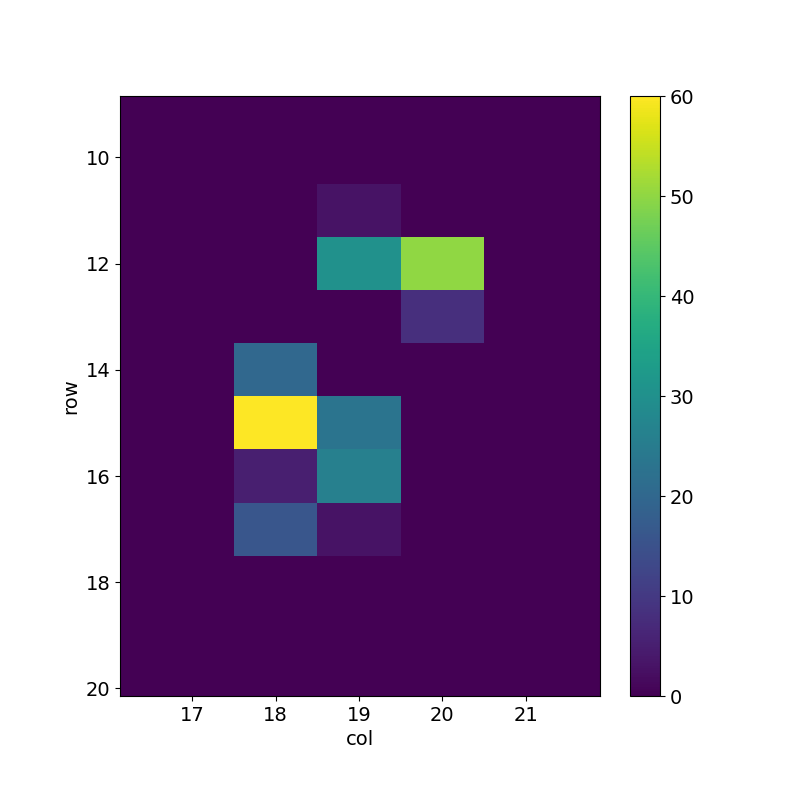
\includegraphics[width=.3\linewidth]{figures/charaterization/evts/cosmic_rays/11a.png}
                    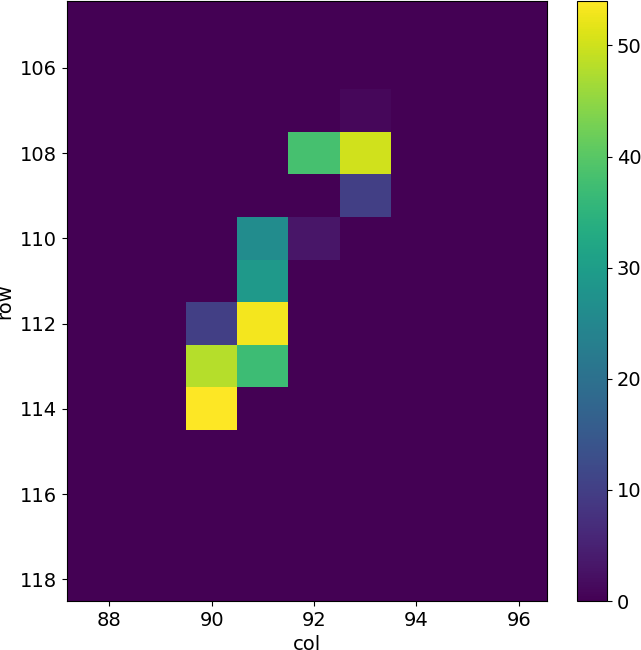
\includegraphics[width=.3\linewidth]{figures/charaterization/evts/cosmic_rays/12.png} 
                    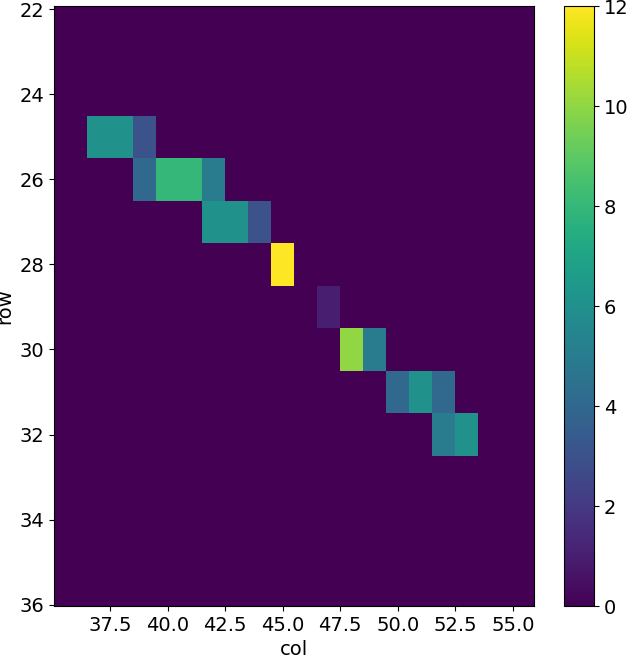
\includegraphics[width=.3\linewidth]{figures/charaterization/evts/cosmic_rays/19a.png}
                \end{figure}

                \begin{itemize}
                    \item Q in cluster is proportional to the cluster size
                    \item broad distribution due to the more various sample of particles and energies
                \end{itemize}
        \end{columns}
    \end{frame}    


    %%%%%%%%%%%%%%%%%%%%%%%%%%%%%%%%%%%%%%%%
    %%  Slide 5: <Dead time>  %%
    %%%%%%%%%%%%%%%%%%%%%%%%%%%%%%%%%%%%%%%%
    \begin{frame}
        \frametitle{Readout time}
        Used the internal \textbf{injection} circuit that allows injecting pulses at different rate 
        \begin{itemize}
            \item No memory on pixel
            \item Readout is completely sequential: one serializer @ \SI{40}{MHz}
            \begin{itemize}
                \item each hit is a 27-bits data packet, at least \SI{675}{ns} needed 
                \item next prototype version, TJ-Monopix2, has a faster serializer \SI{640}{MHz} that removes the limitation in the readout speed 
            \end{itemize}
        \end{itemize}

        \medskip
        \begin{columns}
            \column{0.55\textwidth}              
                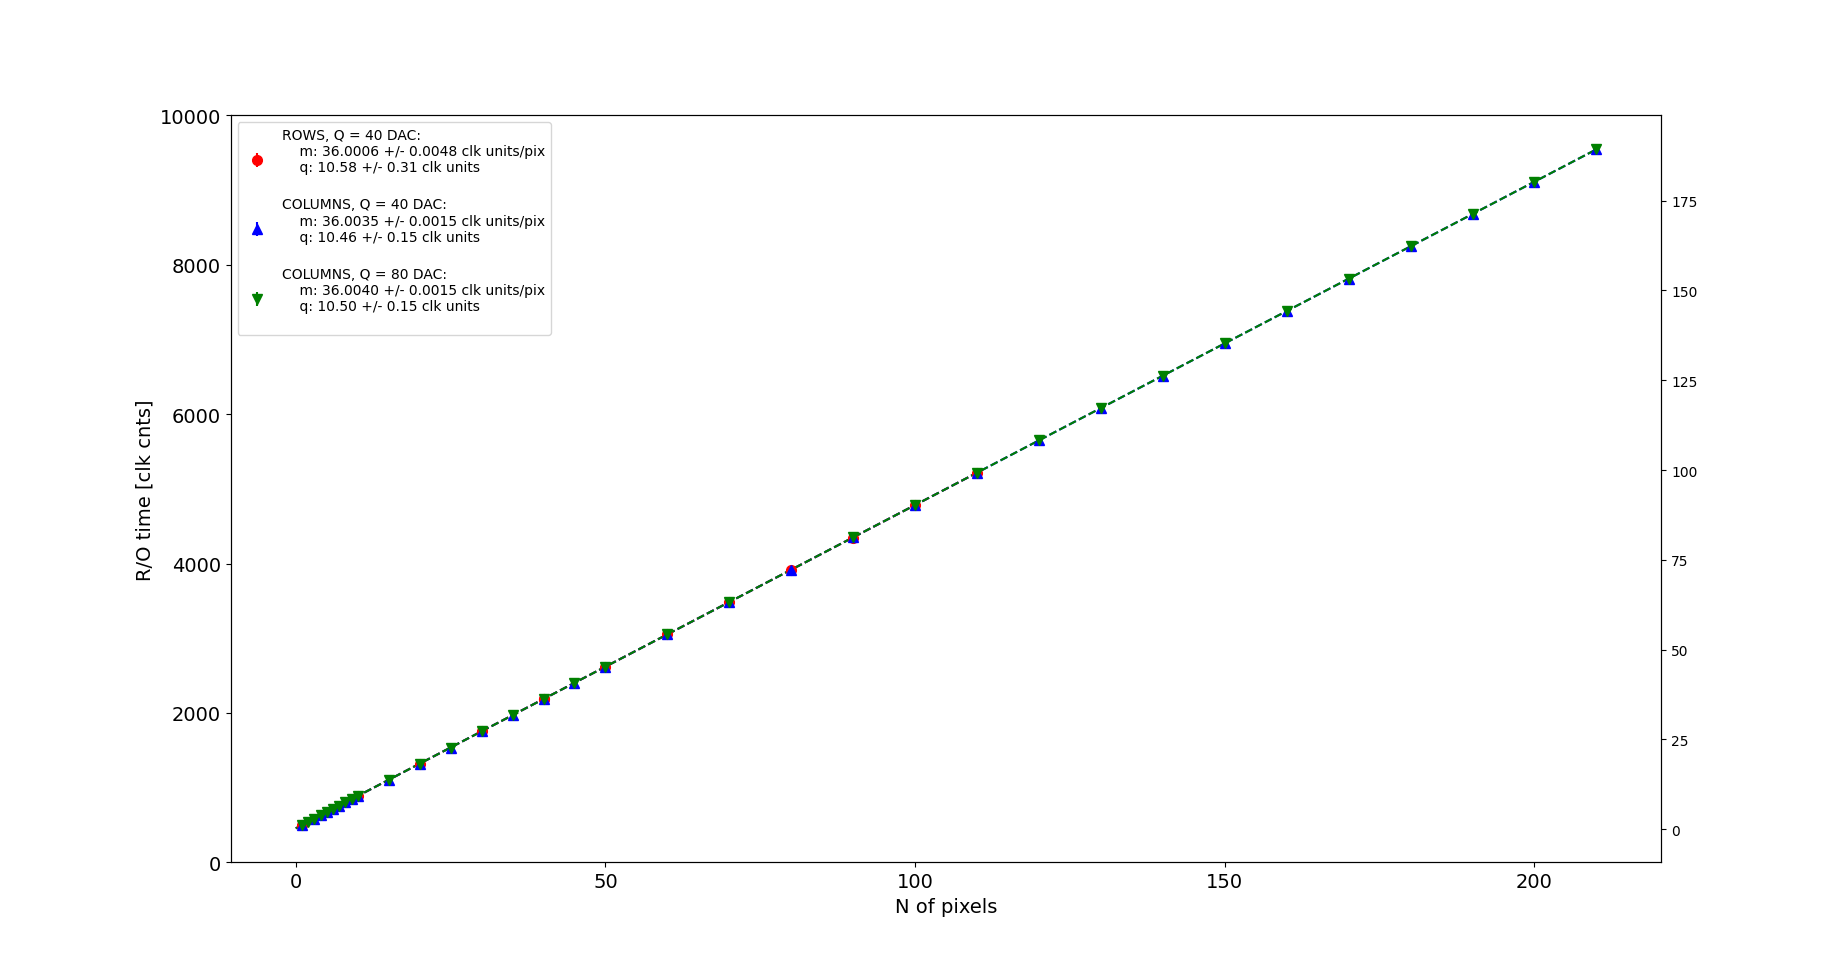
\includegraphics[width=1.07\linewidth]{figures/charaterization/default_line.pdf}
            \column{0.45\textwidth}  
            Readout time \textbf{slightly} depends on the FE status and can be reduced down to \SI{31}{clk.}cnts = \SI{775}{ns} per pixels 

        \end{columns}            
    \end{frame}          